\documentclass[%
 %reprint,
 superscriptaddress,
 %groupedaddress,
 %unsortedaddress,
 %runinaddress,
 %frontmatterverbose,
 preprint,
 showpacs,
 showkeys,
 preprintnumbers,
 %nofootinbib,
 %nobibnotes,
 %bibnotes,
  amsmath,amssymb,
  aps,
 % prl,
 pra,
 %prb,
 % rmp,
 %prstab,
 %prstper,
  longbibliography,
  floatfix,
  %lengthcheck,%
 ]{revtex4-1}
\usepackage{hyperref}

%\documentclass[pra,amsfonts,showpacs,showkeys,preprint,nofootinbib,numerical]{revtex4-1}
\sloppy
\usepackage{graphicx}% Include figure files
\usepackage{epstopdf}
\usepackage{eepic}
\usepackage[dvipsnames]{xcolor}
\usepackage{braket}
\usepackage{amsmath}
\usepackage{amsthm}
\usepackage{tikz}

\RequirePackage{times}
\RequirePackage{mathptm}

%%%%%%%%%%%%%%%%%%%%%%%%%%%%%%%%%%%%%%%%%%%%%%%%%%%%%%%%%%%%%%%%%%%%%%%%%%%

\usepackage{url}
\usepackage{yfonts}

%%%%%%%%%%%%%%%%%%%%%%%%%%%%%%%%%%%%%%%%%%%%%%%%%%%%%%%%%%%%%%%%%%%%%%%%%%%

\theoremstyle{plain}
\newtheorem{theorem}{Theorem}[section]
\newtheorem{lemma}[theorem]{Lemma}
\newtheorem{corollary}[theorem]{Corollary}
\newtheorem{proposition}[theorem]{Proposition}
\newtheorem{definition}[theorem]{Definition}
\newtheorem{remark}[theorem]{Remark}
\newtheorem{example}[theorem]{Example}
\newtheorem{condition}{Condition}
%\newtheorem{algorithm}{Algorithm}

\newtheorem{conjecture}[theorem]{Conjecture}

%%%%%%%%%%%%%%%%%%%%%%%%%%%%%%%%%%%%%%%%%%%%%%%%%%%%%%%%%%%%%%%%%%%%%%%%%%%

\renewcommand{\labelenumi}{(\roman{enumi})}

%%%%%%%%%%%%%%%%%%%%%%%%%%%%%%%%%%%%%%%%%%%%%%%%%%%%%%%%%%%%%%%%%%%%%%%%%%%

\newcommand{\abs}[1]{\left\lvert#1\right\rvert}
\DeclareMathOperator{\Sim}{sim}
\DeclareMathOperator{\Dom}{dom}
\DeclareMathOperator{\arcosh}{arcosh}
%\DeclareMathOperator*{\Limsup}{\varlimsup}
%\DeclareMathOperator*{\Liminf}{\varliminf}

\DeclareMathOperator{\bin}{bin}
\DeclareMathOperator{\Time}{Time}
%\newcommand{\rest}[2]{#1\!\restriction_{#2}}
\newcommand{\rest}[2]{#1\!\!\restriction_{#2}}
\newcommand{\reste}[2]{#1\restriction_{#2}}

\newcommand{\N}{\mathbb{N}}%      \N   == \mathbb{N}
\newcommand{\Z}{\mathbb{Z}}%      \Z   == \mathbb{Z}
\newcommand{\Q}{\mathbb{Q}}%      \Q   == \mathbb{Q}
\newcommand{\R}{\mathbb{R}}%      \R   == \mathbb{R}
%\newcommand{\C}{\mathbb{C}}%      \C   == \mathbb{C}
%\newcommand{\CQ}{\mathbb{C}_Q}%   \CQ  == \mathbb{C}_Q
%\newcommand{\CQ}{\mathbb{Q}(i)}%   \CQ  == \mathbb{Q}(i)
\newcommand{\alphabet}{\{0,1\}}
%\newcommand{\X}{\Sigma^*}%        \X  == \Sigma^*
\newcommand{\B}{B^*}%        \X  == \Sigma^*
%\newcommand{\XI}{\Sigma^\infty}%        \XI  == \Sigma^\infty
\newcommand{\BI}{B^\infty}%        \XI  == \Sigma^\infty
%\newcommand{\K}{H}
%\newcommand{\MK}{\mathcal{H}}
%\newcommand{\OH}{\mathcal{H}}
\newcommand{\OH}{\hat{H}}
\newcommand{\BO}{\mathcal{B}(X)}
%\newcommand{\BO}{\mathfrak{B}(X)
\newcommand{\HO}{\mathcal{B}_h(X)}
%\newcommand{\SAO}{\mathfrak{O}(X)}
\newcommand{\PO}{\mathcal{B}(X)_+}
\newcommand{\x}{\mathbf{x}}
\newcommand{\ar}{\rightarrow}
\DeclareMathOperator{\Pf}{Pf}

%%%%%%%%%%%%%%%%%%%%%%%%%%%%%%%%%%%%%%%%%%%%%%%%%%%%%%%%%%%%%%%%%%%%%%%%%%%

%\DeclareMathOperator{\Prob}{Pr}
%\newcommand{\alp}{\mathcal{H}}
\DeclareMathOperator*{\eqbelow}{=}
\newcommand{\df}{\eqbelow_{\text{def}}}

%%%%%%%%%%%%%%%%%%%%%%%%%%%%%%%%%%%%%%%%%%%%%%%%%%%%%%%%%%%%%%%%%%%%%%%%%%%

\newcommand{\noi}{\noindent}

%%%%%%%%%%%%%%%%%%%%%%%%%%%%%%%%%%%%%%%%%%%%%%%%%%%%%%%%%%%%%%%%%%%%%%%%%%%

\pagestyle{plain}
%%%%%%%%%%%%%%%%%%%%%%%%%%%%%%%%%%%%%%%%%%%%%%%%%%%%%%%%%%%%%%%%%%%%%%%%%%%
%\newcommand{\bra}[1]{\left< #1 \right|}
%\newcommand{\ket}[1]{\left| #1 \right>}

\newcommand{\iprod}[2]{\langle #1 | #2 \rangle}
\newcommand{\mprod}[3]{\langle #1 | #2 | #3 \rangle}
\newcommand{\oprod}[2]{| #1 \rangle\langle #2 |}

\newcommand{\proj}[3]{\begin{smallmatrix} #1 & #2 & #3 \end{smallmatrix}}
\newcommand{\projbf}[3]{\begin{smallmatrix} \mathbf{#1} & \mathbf{#2} & \mathbf{#3} \end{smallmatrix}}

%\parskip .7em %vskip between paragraphs

\newcommand{\seq}[1]{\mathbf{#1}}
\newcommand{\floor}[1]{\left\lfloor #1 \right\rfloor}
\newcommand{\ceil}[1]{\left\lceil #1 \right\rceil}
\newcommand{\m}[1]{\widetilde{#1}}
\newcommand{\xor}{\text{ ${\tt XOR}$ }}
%%%%%%%%%%%%%%%%%%%%%%%%%%%%%%%%%%%%%%%%%%%%%%%%%%%%%%%%%%%%%%%%%%%%%%%%%%%


%\usepackage{cdmtcs}
\begin{document}


\title{Value Indefiniteness Is Almost Everywhere}
%Strong Kochen-Specker Theorem and The Logical Indeterminacy Principle}

\author{Alastair A. Abbott}
\email{a.abbott@auckland.ac.nz}
\homepage{http://www.cs.auckland.ac.nz/~aabb009}

\affiliation{Department of Computer Science, University of Auckland,
Private Bag 92019, Auckland, New Zealand}
\affiliation{Centre Cavaill\`es, CIRPHLES, \'Ecole Normale Sup\'erieure, 29 rue d'Ulm, 75005 Paris, France}

\author{Cristian S. Calude}
\email{cristian@cs.auckland.ac.nz}
\homepage{http://www.cs.auckland.ac.nz/~cristian}


\affiliation{Department of Computer Science, University of Auckland,
Private Bag 92019, Auckland, New Zealand}


\author{Karl Svozil}
\email{svozil@tuwien.ac.at}
\homepage{http://tph.tuwien.ac.at/~svozil}

\affiliation{Institute for Theoretical Physics,
Vienna  University of Technology,
Wiedner Hauptstrasse 8-10/136,
1040 Vienna,  Austria}

\date{\today}

\begin{abstract}
%Kochen-Specker type theorems assure the breakdown of certain non-contextual hidden variable theorems through the non-existence of global, holistic frame functions;
%alas they do not target the location and the extent of this phenomenon.
%Here we show the strongest conceivable form of quantum indeterminacy---sometimes also referred to as contextuality or value indefiniteness---by proving that, once a single arbitrary observable is fixed to be value definite, almost (i.e.\ with Lebesgue measure one) all remaining observables are indeterminate relative to the assumptions, in particular that any value assignments must necessarily be non-contextual.

Kochen-Specker  theorems assure the breakdown of certain types of non-contextual hidden variable theorems through the non-existence of global, holistic frame functions;
alas they do not allow us to identify where this breakdown occurs, nor the extent of it.
Here we show that this breakdown is maximal in that it occurs almost everywhere, and thus prove that quantum indeterminacy---often referred to as contextuality or value indefiniteness---is a global property as is often assumed.
In contrast to the Kochen-Specker theorem, we assume only weak constraints on any definite values that may exist, in particular that any potential value assignments that may exist be locally non-contextual.
Under this assumption, we prove that once a single arbitrary observable is fixed to be value definite, almost (i.e. with Lebesgue measure one) all remaining observables are indeterminate.
%Specifically, we prove that once a single arbitrary observable is fixed to be value definite, almost (i.e. with Lebesgue measure one) all remaining observables are indeterminate if weak constraints on any definite values that may exist are required, in particular that any potential value assignments that may exist be locally non-contextual.
\end{abstract}

\pacs{03.67.Lx, 05.40.-a, 03.65.Ta, 03.67.Ac, 03.65.Aa}
\keywords{Kochen-Specker theorem, quantum value indefiniteness, quantum randomness, logical indeterminacy principle, quantum contextuality}
\preprint{CDMTCS preprint nr. 443}
\maketitle

\section{Introduction}
The Kochen-Specker theorem \cite{specker-60,kochen1}
proves the impossibility of the existence of certain hidden variable theories for quantum mechanics by showing the existence of a finite set of observables $\mathcal{O}$ for which  the following two assumptions cannot be simultaneously true:
\begin{itemize}
        \item[(P1)]
        every observable in $\mathcal{O}$  has a pre-assigned definite value,
        \item[(P2)]
        the outcomes of measurements of observables are non-contextual.
\end{itemize}

 Non-contextuality means that the outcomes of measurements of observables
are independent of whatever other
co-measurable observables are measured alongside them,
along with the requirement that the relationship between hidden variables associated with
sets of co-measurable observables behave quasi-classically, as expected from quantum mechanics.
This requirement means that in any ``complete, maximal'' set of mutually co-measurable yes-no propositions
(represented by mutually orthogonal projectors spanning the Hilbert space, or, equivalently, by a single ``maximal'' operator with a spectral decomposition containing these projectors)
exactly one proposition should be assigned the value ``yes.''
Due to complementarity, the observables in $\mathcal{O}$ may not be all simultaneously co-measurable, that is, formally, commuting.

The Kochen-Specker theorem  {\em does not explicitly identify}
certain particular observables which violate one or both assumptions (P1) and (P2), but only proves their {\em existence}.
This form of the theorem was amply sufficient for its intended scope, primarily metaphysical.
The relation between  value indefinite observables, that is, observables which do not have definite values before measurement,
and quantum randomness in \cite{specker-60,kochen1}, requires a more  precise form of the Kochen-Specker theorem in which some value indefinite observables can be located (identified). A stronger form of the Kochen-Specker theorem providing this information was proved in \cite{2012-incomput-proofsCJ}.

In this paper we extend these results
% results of \cite{2012-incomput-proofsCJ}, which provide a subset of observables which can be identified as value indefinite,
to show that indeed all observables must be value indefinite except for those corresponding to the context used to prepare the state.
While it may seem intuitive that quantum indeterminism is this widespread, it does not follow from existing no-go theorems, so it is important that a theoretical grounding be given to this intuition.
This not only helps provide an information theoretic certification of quantum random bits, but also develops our understanding of the origin of quantum indeterminism.

\section{Logical indeterminacy principle}
Pitowsky \cite{pitowsky:218} (also in the subsequent paper \cite{hru-pit-2003} with Hrushovski) gave a constructive proof of Gleason's lemma in terms of orthogonality graphs which motivated the study of probability distributions on finite sets of rays. In this context he proved a result called ``the logic indeterminacy principle'' which has a striking similarity with the Kochen-Specker theorem and appears as if it could be used to locate value indefiniteness.
However, as we discuss in this section this is not the case.

According to \cite{hru-pit-2003}, a \emph{frame function} on a set $\mathcal{O}\subset \mathbb{C}^n$ of projection observables (which we identify here with the unit vectors they project on to) in a dimension $n\ge 3$ Hilbert space is a function $p:\mathcal{O}\to [0,1]$ such that:
\begin{enumerate}
	\item If $\{\ket{x_1},\dots,\ket{x_n}\}$ is an orthonormal basis, $\sum_{i=1}^n p(\ket{x_i})=1$, and for $\{\ket{x_1},\dots,\ket{x_k}\}$ orthonormal with $k\le n$, $\sum_{i=1}^k p(\ket{x_i})\le 1$.
	\item For all complex $\alpha$ with $|\alpha|=1$ and all $x\in O$, $p(\ket{x})=p(\alpha \ket{x})$.
\end{enumerate}

A {\em Boolean frame function} is a frame function taking only $0,1$ values, i.e.\ for all $\ket{x}\in\mathcal{O}$, $p(\ket{x})\in\{0,1\}$.

\begin{theorem}[Logical indeterminacy principle; Pitowsky \cite{pitowsky:218}]
%%%%CC Let $p$ be a Boolean frame function.
For all projectors $a,b \in \mathbb{C}^{3}$ with $0<|\langle a|b\rangle| < 1$,
there exists a finite set of observables $\mathcal{O}$ with $\ket{a},\ket{b} \in \mathcal{O}$
such that there is no Boolean frame function $p$ on $\mathcal{O}$ unless $p(\ket{a})=p(\ket{b})=0$.
\end{theorem}

%The theorem states that for every two distinct non-orthogonal unit vectors  $\ket{a}, \ket{b}\in \mathbb{C}^{3}$
%there exists a finite set of observables $\mathcal{O}$ such that there is a Boolean frame function $p$ on $\mathcal{O}$ only if
%$p(\ket{a})=p(\ket{b})=0$.
A consequence of this principle is that there is no Boolean frame function $p$ on $\mathcal{O}$ such that $p(\ket{a})=1$. From the  logical indeterminacy principle we can deduce the Kochen-Specker theorem
because a Boolean frame function simply gives a non-contextual,
value definite %on $\mathcal{O}$
yes-no value assignment, so  (P2) is satisfied.

As noted by Hrushovski and Pitowsky \cite{hru-pit-2003},  the  logical indeterminacy principle  is stronger than the Kochen-Specker theorem because the result is true for arbitrary frame functions which can take every value in the unit interval $[0,1]$, but which are restricted to Boolean values for $\ket{a},\ket{b}$.

In fact, we may be tempted to use the  logical indeterminacy principle  to ``locate'' a
value indefinite observable. Indeed, if we fix $p$ and  choose $\ket{a} \in \mathbb{C}^{3}$ such that
$p(\ket{a})=1$, then, by the  logical indeterminacy principle, for every distinct non-orthogonal unit vector $\ket{b} \in \mathbb{C}^{3}$
it is impossible to have  $p(\ket{b})=1$ and $p(\ket{b})=0$, hence one could be inclined to conclude that $\ket{b}$ is value indefinite.
However, such reasoning would be incorrect because if $p(\ket{b})$ were $1$, then the  logical indeterminacy principle merely
concludes that $p$ {\em does not exist};
the same conclusion is obtained if $p(\ket{b})$ were $0$. Hence, in both cases $p$ {\em does not exist},
so it makes no sense to talk about its values, in particular, about $p(\ket{b})$.
(Pointedly stated from a physical viewpoint, $p(\ket{a})$ as well as $p(\ket{b})$ could take on any of the four combinations of definite values, provided that
(P1) or (P2) is violated for some other observable in $\mathcal{O}$.
Nevertheless, as we shall demonstrate in Section~\ref{sec:main}, using the formalism of \cite{2012-incomput-proofsCJ},
all observables in $\mathcal{O}$ except $\ket{a}$ and those commuting with $\ket{a}$ are indeed provable value indefinite.)
This means that using the  logical indeterminacy principle we get the same global information derived in the Kochen-Specker theorem,
namely that some observable in $\mathcal{O}$ has to be value indefinite, and no more.
The reason for this limitation is the use of  frame functions, which by definition must be defined everywhere: they can model
``local'' value definiteness, but not  ``local''
value indefiniteness, which, as in the Kochen-Specker theorem, ``emerges'' only as a global phenomenon.

\section{Value indefiniteness and contextuality }
 To remedy the above deficiency we will use the formalism proposed in \cite{2012-incomput-proofsCJ}
for pure quantum states. Specifically, we define value (in)definiteness and contextuality in the framework of quantum logic of Birkhoff and von Neumann \cite{v-neumann-55,birkhoff-36}
and Kochen and Specker \cite{kochen2,kochen3}.

Projection operators---projecting on to the linear subspace spanned by a non-zero vector $\ket{\psi}$---will be denoted by  $P_\psi = \frac{\oprod{\psi}{\psi}}{\iprod{\psi}{\psi}}\raisebox{.8mm}{.}$

\medskip


We fix a positive integer $n$.
Let $\mathcal{O} \subseteq \{ P_\psi \mid \ket{\psi} \in \mathbb{C}^n \}$ be a non-empty set of {\em projection observables} in the Hilbert space $\mathbb{C}^n$ and $\mathcal{C}\subseteq \{\{P_1,P_2,\dots P_n\} \mid P_i \in \mathcal{O} \text{ and } \iprod{i}{j}=0 \text{ for } i\neq j \}$ a set of measurement contexts over $\mathcal{O}$.
A {\em context} $C\in\mathcal{C}$ is thus a maximal set of compatible (i.e.\ they can be simultaneous measured) projection observables.
Let $v : \{(o,C) \mid o\in \mathcal{O}, C\in\mathcal{C}\text{ and } o\in C \} \xrightarrow{o} \{0,1\}$ be a partial function
(i.e., $v$ may be undefined for some values in its domain)  called an \emph{assignment function}.
For some $o,o'\in \mathcal{O}$ and $C,C'\in\mathcal{C}$ we say $v(o,C)=v(o',C')$ if $v(o,C),v(o',C')$ are both defined and have equal values.
%If either $v(o,C)$ or $v(o',C')$ are not defined or they are both defined but have different values, then $v(o,C)\neq v(o',C')$.
%The \emph{assignment function} $v$   specifies in advance the result obtained from the measurement of an observable.

\medskip

 Value definiteness corresponds to the %classical notion of determinism:
  notion of predictability in classical determinism:
an observable is value definite if $v$ assigns it a definite value---i.e.\ is able to predict in advance, independently of measurement,  the value obtained via measurement. Here is the formal definition: an
 observable $o\in C$ is \emph{value definite} in the context $C$ under $v$ if $v(o,C)$ is defined;
otherwise $o$ is \emph{value indefinite} in $C$.
If $o$ is value definite in all contexts $C\in \mathcal{C}$ for which $o\in C$ then we simply say that $o$ is value definite under $v$.
%Similarly, if $o$ is value indefinite in all such contexts $C$ then we say that $o$ is value indefinite under $v$.
The set $\mathcal{O}$ is \emph{value definite} under $v$ if every observable $o\in\mathcal{O}$ is value definite under $v$.
This fine-grained definition of value definiteness allows us to formalise located value (in)definiteness, which one cannot do with the global notion used in the Kochen-Specker theorem.

\medskip

Non-contextuality corresponds to the classical notion that the value obtained via measurement is independent of other compatible observables measured alongside it. Formally, an
 observable $o\in \mathcal{O}$ is \emph{non-contextual} under $v$ if for all contexts $C,C' \in \mathcal{C}$ with $o\in C,C'$ we have $v(o,C)=v(o,C')$; otherwise, $v$ is \emph{contextual}.
%Note that an observable which is value indefinite in a context is always contextual even if it takes the same value in every context in which it is value definite.
%On the other hand, if an observable is value definite in all contexts that it is in, it can be either contextual or not (and in the latter case its value is constant in all contexts containing it) depending on $v$.
The set of observables $\mathcal{O}$ is \emph{non-contextual} under $v$ if every observable $o\in\mathcal{O}$ which is not value indefinite (i.e.\ value definite in \emph{some} context) is non-contextual under $v$;
otherwise, the set of observables $\mathcal{O}$ is \emph{contextual}.
Thus we require that {\em observables behave non-contextually only where definite values are defined}; this technicality is necessary in order to consider the possibility that some observables are value indefinite.
%Further, we say that the set of observables $\mathcal{O}$ is \emph{strongly contextual} under $v$ if every observable $o\in\mathcal{O}$ is contextual under $v$.
%Every strongly contextual set of observables under $v$ is contextual under $v$, provided that $v$ is not undefined everywhere;
%however the converse implication is false
%If an observable $o$ is non-contextual then it is value definite, but this is not true for sets of observables: $\mathcal{O}$ can be non-contextual but not value definite if it contains an observable which is value indefinite.

\medskip


To be in agreement with quantum mechanics we restrict the assignment functions to admissible ones:   $v$ is  \emph{admissible} if the following hold for all $C \in \mathcal{C}$: a)
if there exists an $o\in C$ with $v(o,C)=1$, then $v(o',C)=0$ for all $o'\in C\setminus\{o\}$, b)
if there exists an $o\in C$ such that $v(o',C)=0$ for all $o'\in C\setminus \{o\}$, then $v(o,C)=1$.




\section{Strong Kochen-Specker theorem}

The incompatibility between the assumptions (P1)  and (P2) is not {\em maximal} in the following sense: for any set of contexts over any set of observables, there exists an admissible assignment function under which the set of observables is value definite and at least one observable is non-contextual.

However, {\em there always exist pairs of observables such that, if one of them is assigned the value $1$ by an admissible assignment function under which $\mathcal{O}$ is non-contextual, the other must be {\rm value indefinite}.} The result is deduced in \cite{2012-incomput-proofsCJ}  using the weaker assumption that  not all observables are assumed to be value definite:
{\em An observable is deduced to be value definite only when the values of other commuting value-definite observables require it to be so}; this is expressed formally by the admissibility of $v$.
%{\em An observable is deduced to be value definite only where the specific requirements of the admissibility of $v$ requires it to be so}.


\begin{lemma}[Strong Kochen-Specker lemma; \cite{2012-incomput-proofsCJ}]
\label{thm:twonotvalueone}
        Let $\ket{a}, \ket{b}\in \mathbb{C}^3$ be unit vectors such that $0 < |\iprod{a}{b}| \le \frac{3}{\sqrt{14}}\raisebox{.8mm}{.}$
        Then there exists a set of 24 projection observables $\mathcal{O}$ containing $P_a$ and $P_b$, and a set of contexts $\mathcal{C}$ over $\mathcal{O}$, such that there is no admissible assignment function under which $\mathcal{O}$ is non-contextual and $P_a$, $P_b$ have the value $1$.
\end{lemma}


The strong Kochen-Specker theorem can be used to ``locate'' a provable value indefinite observable which when measured ``produces'' a quantum random bit whose quality can be precisely evaluated under some physical assumptions:

\begin{theorem}[Strong Kochen-Specker theorem; \cite{2012-incomput-proofsCJ}]
\label{thm:twonotvaluedefinite}
        Let $\ket{a}, \ket{b}\in \mathbb{C}^3$ be unit vectors such that $\sqrt{\frac{5}{14}} \le |\iprod{a}{b}| \le \frac{3}{\sqrt{14}}\raisebox{.8mm}{.}$
        Then there exists a set of 24 projection observables $\mathcal{O}$ containing $P_a$ and $P_b$, and a set of contexts $\mathcal{C}$ over $\mathcal{O}$, such that there is no admissible assignment function under which $\mathcal{O}$ is non-contextual, $P_a$ has the value $1$ and $P_b$ is value definite.
\end{theorem}


\section{How widespread is value indefiniteness?}
\label{sec:main}
%The natural question which remains to be answered is the following.
%Assuming that $P_a$ has the value 1, we know that $P_b$ is value indefinite.
%In this section we address the following question: %which of the remaining 22 projection observables in $\mathcal{O}$ can be value definite?
Assuming an observable $P_a$ has the value 1 we know we can find an observable $P_b$ that is value indefinite.
In this section we address the following question: which of the remaining observables $P_b$ can be proven to be value indefinite?
We prove here the following answer, showing the extent of value indefiniteness: {\em only observables which commute with $P_a$ can be value definite}.
Specifically, we will prove the following, more general, theorem which extends the Strong Kochen-Specker theorem to cover the rest of the Bloch sphere.

\begin{theorem}
\label{thm:twonotvaluedefiniteUltimate}
        Let $\ket{a}, \ket{b}\in \mathbb{C}^3$ be non orthogonal or parallel unit vectors, i.e. $0 < |\iprod{a}{b}| < 1$.
        Then there exists a set of projection observables $\mathcal{O}$ containing $P_a$ and $P_b$, and a set of contexts $\mathcal{C}$ over $\mathcal{O}$, such that there is no admissible assignment function under which $\mathcal{O}$ is non-contextual, $P_a$ has the value 1 and $P_b$ is value definite. The set $\mathcal{O}$ is finite and can be effectively constructed.
\end{theorem}

While this result is similar in form to the original Kochen-Specker theorem, the subtle differences are critical.
As mentioned previously, the Kochen-Specker theorem is unable to locate value definiteness: if $P_a$ has the value 1, we cannot conclude that $P_b$ is value indefinite, even if assigning it leads to a contradiction.
This is due to the fact that this contradiction implies only that no \emph{global} assignment function can exist; the Kochen-Specker theorem does not show that $P_b$ could not be value definite, while some other $P_c$ harbours the (necessary) value indefiniteness.

On the other hand, the sets of observables given in the proofs of the Strong Kochen-Specker theorems presented here
are carefully constructed such that any attempt to place the value indefiniteness on a $P_c$ necessarily contradicts the admissibility of $v$.
For example, it would require a context containing an observable assigned the value 1, and another observable being value indefinite.
This contradicts both the the admissibility of $v$, and the physical understanding of what it means for that observable to be assigned the value 1---since we know measuring that observable will give the value 1, measuring the other observables \emph{must} give the value 0, and hence the other observables are necessarily value definite.
As a result, we are forced to conclude that $P_b$ itself is value indefinite.


In order to prove Lemma~\ref{thm:twonotvalueone}, in \cite{2012-incomput-proofsCJ} a specific proof for the case  $|\iprod{a}{b}|=\frac{3}{\sqrt{14}}$ was given, followed by a reduction to this proof for the case $|\iprod{a}{b}|<\frac{3}{\sqrt{14}}.$
Here we prove the theorem holds for all cases by reducing
%Here we show a reduction for
the remaining case of $|\iprod{a}{b}|>\frac{3}{\sqrt{14}}$ to the existing result.
This reduction is more subtle and difficult than the first one.
%%%%CC for the  case proven in \cite{2012-incomput-proofsCJ}.

For the purpose of illustrating the reduction technique, let us state the following lemma from \cite{2012-incomput-proofsCJ}, which will also turn out to be important for the reduction we will give here.

\begin{lemma}
	\label{lemma:reduction1}
%%%%CC 	Given any two unit vectors $\ket{a},\ket{b}$ with $0 < |\iprod{a}{b}| < 1$, there
%%%%CC exists for every $x$ such that $|\iprod{a}{b}| < |x| < 1$ a unit vector $\ket{c}$ with $
Given any two unit vectors $\ket{a},\ket{b}$ with $0 < |\iprod{a}{b}| < 1$ and an $x$ such that $|\iprod{a}{b}| < |x| < 1$, there exist a unit vector $\ket{c}$ with $
\iprod{a}{c}=x$, a set of observables $\mathcal{O}$ containing $P_a,P_b,P_c$ and a set of contexts $\mathcal{C}$ over $\mathcal{O}$ such that if $P_a$ and $P_b$ have the value 1, then $P_c$ also has the value 1 under any admissible, non-contextual assignment function on $\mathcal{O}$.
	
	Furthermore, if we choose our basis such that $\ket{a}\equiv (1,0,0)$ and $\ket{b}\equiv(p,q,0)$, where $p=\iprod{a}{b}$ and $q=\sqrt{1-p^2}$, then $\ket{c}$ has the form $\ket{c}=(x,y,\pm z)$, where $x=\iprod{a}{c}$, $y=\frac{p(1-x^2)}{qx}$ and $z=\sqrt{1-x^2-y^2}$.
\end{lemma}
This lemma is illustrated in Fig.~\ref{fig:reduction2} and constitutes a simple ``forcing'' of value definiteness: given $P_a$ and $P_b$ both with the value 1, there is a $P_c$ which is ``closer'' (i.e. at a smaller angle of our choosing) to $P_a$ which forces $P_c$ to also take the value 1.

\begin{figure}[t]
\begin{center}
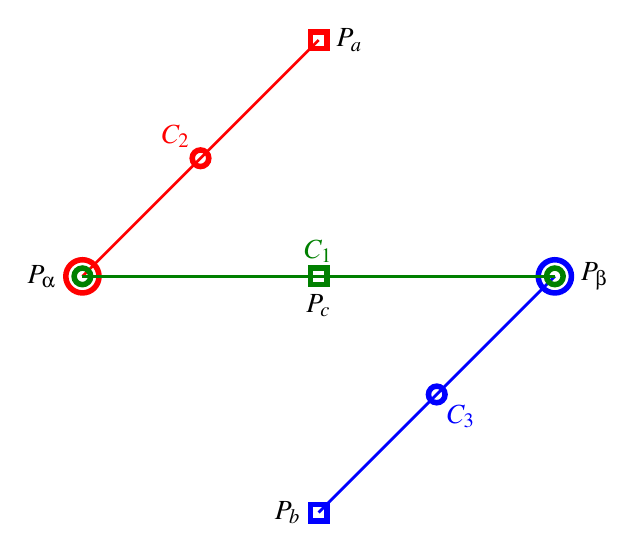
\begin{tikzpicture}
\tikzstyle{every path}=[line width=1pt]
\tikzstyle{every node}=[draw,line width=2pt,inner sep=0]

\tikzstyle{y1}=[rectangle,minimum size=6]

\tikzstyle{n1}=[circle,minimum size=6]
\tikzstyle{n2}=[circle,minimum size=12]

\tikzstyle{l1}=[draw=none,rectangle,minimum size=9]
\tikzstyle{l2}=[draw=none,rectangle,minimum size=15]

\draw[Red] (90:3) -- (180:3)
        coordinate[y1,at start] (a)
        coordinate[n1,midway,label=135:$C_2$] (0 y z)
        coordinate[n2,at end] (alpha);

\draw[Blue] (270:3) -- (0:3)
        coordinate[y1,at start] (b)
        coordinate[n1,midway,label=315:$C_3$] (q -p ?)
        coordinate[n2,at end] (beta);

\draw[Green] (alpha.center) -- (beta.center)
        coordinate[n1,at start] (alpha)
        coordinate[y1,midway,label=90:$C_1$] (c)
        coordinate[n1,at end] (beta);

\coordinate[l1,label=0:$P_a$] (a) at (a.center);
\coordinate[l1,label=180:$P_b$] (b) at (b.center);

\coordinate[l2,label=180:$P_\alpha$] (alpha) at (alpha.center);
\coordinate[l2,label=0:$P_\beta$] (beta) at (beta.center);

\coordinate[l1,label=270:$P_c$] (c) at (c.center);
\end{tikzpicture}
\end{center}
\caption{(Color online) Greechie orthogonality diagram with an overlaid value assignment that illustrates the reduction in Lemma~\ref{lemma:reduction1}.
         The circles and squares represent observables that will be given the values $0$ and $1$ respectively.
         They are joined by smooth lines which represent contexts.}
\label{fig:reduction1}
\end{figure}

This reduction, however, requires necessarily that $|x|>|p|$, and finding a reduction to ``force'' in the other direction (i.e. towards larger angles between $P_a$ and $P_c$) is difficult.
Here we give an iterated reduction for this case in the following lemma.

\begin{lemma}
	\label{lemma:reduction2}
	Given any two unit vectors $\ket{a},\ket{b}$ with $\frac{3}{\sqrt{14}} < \iprod{a}{b} < 1$, there exists
%%%%CC  exists
	a unit vector $\ket{c}$ with $\iprod{a}{c}\le\frac{3}{\sqrt{14}}$,
	 a set of observables $\mathcal{O}$ containing $P_a,P_b,P_c$ and a set of contexts $\mathcal{C}$ over $\mathcal{O}$ such that if $P_a$ and $P_b$ have the value 1, then $P_c$ also has the value 1 under any admissible, non-contextual assignment function on $\mathcal{O}$.
\end{lemma}

The proof of this lemma is based on the generalisation of a specific reduction for the case of $\iprod{a}{b}=\frac{1}{\sqrt{2}}$ to $\iprod{a}{c}=\frac{1}{\sqrt{3}}$; i.e. it is a ``forcing'' argument in the required direction. The Greechie diagram for this is depicted in Fig.~\ref{fig:reduction2}.
In essence, this figure consists of three copies of the reduction shown in Fig.~\ref{fig:reduction1} glued together, ensuring that the Greechie diagram is indeed realisable. Specifically, the important relations are: $\iprod{a}{v_1}=\sqrt{\frac{2}{3}}\raisebox{0.5ex}{,}$ $\iprod{a}{v_2}=\frac{2}{\sqrt{5}}\raisebox{0.5ex}{,}$ $\iprod{b}{c}=\sqrt{\frac{2}{3}}$ and $\iprod{b}{v_2}=\sqrt{\frac{2}{5}}\raisebox{0.5ex}{.}$
The angles between unit vectors in this proof are then scaled, in a way which we will soon make precise, to fit the required $\iprod{a}{b}$ for the general case.
However, since this doesn't allow us to assert that an arbitrary $\ket{c}$ must have the value 1 in the same way we could using Lemma~\ref{lemma:reduction1}, this reduction is then iterated a finite number of times until a sufficiently small $\iprod{a}{c}$ is obtained.

\begin{figure}[t]
\begin{center}
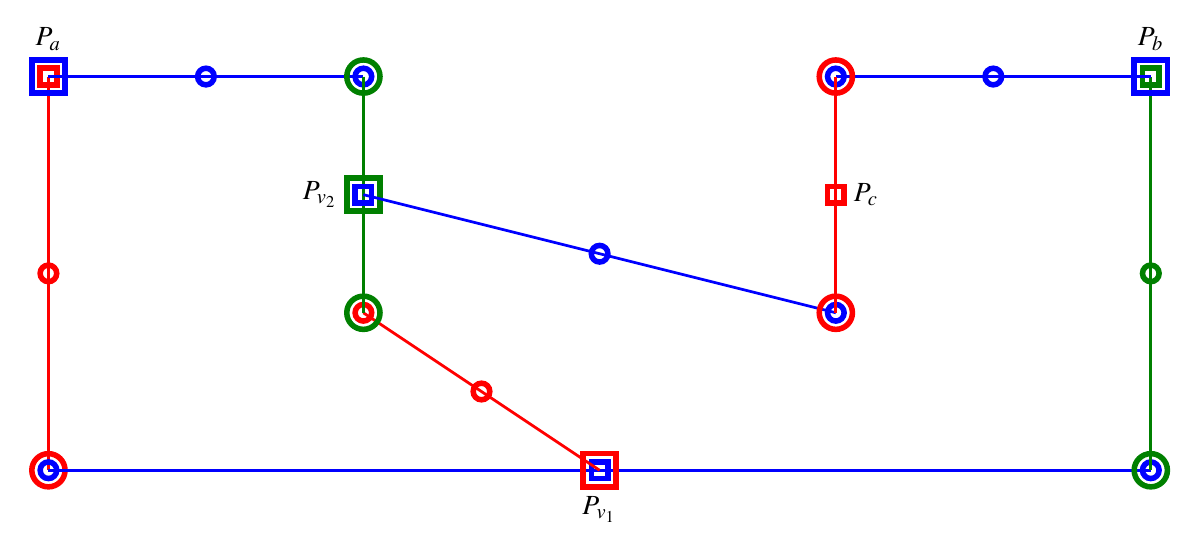
\begin{tikzpicture}
\tikzstyle{every path}=[line width=1pt]
\tikzstyle{every node}=[draw,line width=2pt,inner sep=0]

\tikzstyle{y1}=[rectangle,minimum size=6]
\tikzstyle{y2}=[rectangle,minimum size=12]

\tikzstyle{n1}=[circle,minimum size=6]
\tikzstyle{n2}=[circle,minimum size=12]

\tikzstyle{l1}=[draw=none,rectangle,minimum size=9]
\tikzstyle{l2}=[draw=none,rectangle,minimum size=15]

\draw[Red] (0,5) -- (0,0)
        coordinate[y1,at start] (a)
        coordinate[n1,midway] (d1)
        coordinate[n2,at end] (av1);

\draw[Blue] (av1.center) -- (14,0)
        coordinate[n1,at start] (av1)
        coordinate[y1,midway] (v1)
        coordinate[n1,at end] (bv1);

\draw[Green] (bv1.center) -- (14,5)
        coordinate[n2,at start] (bv1)
        coordinate[n1,midway] (d2)
        coordinate[y1,at end] (b);
		
\draw[Blue] (a.center) -- (4,5)
        coordinate[y2,at start] (a)
        coordinate[n1,midway] (d3)
        coordinate[n1,at end] (av2);
		
\draw[Red] (v1.center) -- (4,2)
        coordinate[y2,at start] (v1)
        coordinate[n1,midway] (d4)
        coordinate[n1,at end] (v1v2);
		
\draw[Green] (av2.center) -- (v1v2.center)
        coordinate[n2,at start] (av2)
        coordinate[y2,midway] (v2)
        coordinate[n2,at end] (v1v2);
		
\draw[Blue] (b.center) -- (10,5)
        coordinate[y2,at start] (b)
        coordinate[n1,midway] (d5)
        coordinate[n1,at end] (bc);
		
\draw[Blue] (v2.center) -- (10,2)
        coordinate[y1,at start] (v2)
        coordinate[n1,midway] (d6)
        coordinate[n1,at end] (v2c);
		
\draw[Red] (v2c.center) -- (bc.center)
        coordinate[n2,at start] (v2c)
        coordinate[y1,midway] (c)
        coordinate[n2,at end] (bc);

\coordinate[l2,label=90:$P_a$] (a) at (a.center);
\coordinate[l2,label=90:$P_b$] (b) at (b.center);
\coordinate[l1,label=0:$P_c$] (c) at (c.center);
\coordinate[l2,label=270:$P_{v_1}$] (v1) at (v1.center);
\coordinate[l2,label=180:$P_{v_2}$] (v2) at (v2.center);

%\coordinate[l2,label=180:$P_\alpha$] (alpha) at (alpha.center);
%\coordinate[l2,label=0:$P_\beta$] (beta) at (beta.center);

%\coordinate[l1,label=270:$P_c$] (c) at (c.center);
\end{tikzpicture}
\end{center}
\caption{(Color online) Greechie orthogonality diagram with an overlaid value assignment that illustrates the reduction in Lemma~\ref{lemma:reduction2}.
         %The circles and squares represent observables that will be given the values $0$ and $1$ respectively.
        % They are joined by smooth lines which represent contexts.
		}
\label{fig:reduction2}
\end{figure}


\begin{proof}[Proof of Lemma~\ref{lemma:reduction2}]
	The constants which will be used for scaling, obtained from the reduction shown in Fig.~\ref{fig:reduction2}, are as follows:
	$$
	\alpha_1=\frac{\arccos\sqrt{\frac{2}{3}}}{\arccos\frac{1}{\sqrt{2}}}\raisebox{0.5ex}{,}\phantom{xxx}
	\alpha_2=\frac{\arccos\frac{2}{\sqrt{5}}}{\arccos\sqrt{\frac{2}{3}}}\raisebox{0.5ex}{,}\phantom{xxx}
	\alpha_3=\frac{\arccos\sqrt{\frac{2}{3}}}{\arccos\sqrt{\frac{2}{5}}}\raisebox{0.5ex}{.}	$$
	Given the initial $\ket{a}$, $\ket{b}$ and the above constants, we thus make use of the following scaled angles between the relevant observables:
	$$
	\theta_{a,b}=\arccos\iprod{a}{b},\phantom{xxx}
	\theta_{a,v_1}=\alpha_1 \theta_{a,b},\phantom{xxx}
	\theta_{a,v_2}=\alpha_2 \theta_{a,v_1}.
	$$
	Once $\ket{v_2}$ is determined via the procedure to follow, we take the following:
	$$
	\theta_{b,v_2}=\arccos\iprod{b}{v_2},\phantom{xxx}
	\theta_{b,c}=\alpha_3 \theta_{b,v_2}.
	$$


	Without loss of generality, let $\ket{a}=(1,0,0)$ and $\ket{b}=(p_1,q_1,0)$ where $p_1=\iprod{a}{b}$ and $q_1=\sqrt{1-p_1^2}$.
	This fixes our basis for the rest of the reduction.
	We want to have $\ket{v_1}$ such that $\iprod{a}{v_1}=x_1=\cos\theta_{a,v_1}$.
	From Lemma~\ref{lemma:reduction1} we know this is possible since $x_1>p_1$ (because $\alpha_1 < 1$),
	and we have $\ket{v_1}=(x_1,y_1,z_1)$, $y_1=\frac{p_1(1-x_1^2)}{q_1 x_1}$ and $z_1=\sqrt{1-x_1^2-y_1^2}$.

	We now want $\ket{v_2}$ such that $\iprod{a}{v_2}=x_2=\cos\theta_{a,v_2}$ (this is possible since $\alpha_2 < 1$).
	In order to use the same general form (specified in Lemma~\ref{lemma:reduction1}) as above, we perform a change of basis to bring $\ket{v_1}$ into the $xy$-plane, describe $\ket{v_2}$ in this basis using the above result, then perform the inverse change of basis.
	Our new basis vectors are given by $\ket{e_2}=(1,0,0)$, $$\ket{f_2}=(\ket{v_1}-x_1\ket{e_2})/q_2=(0,y_1/q_2,z_1/q_2)$$ where $q_2=\sqrt{1-x_1^2}$, and
	$\ket{g_2}=\ket{e_2}\times\ket{f_2}=(0,z_1/q_2,-y_1/q_2)$.
	We thus have the transformation matrix
	$$T_2=
	\begin{pmatrix}
		1 & 0 & 0\\
		0 & y_1/q_2 & z_1/q_2\\
		0 & z_1/q_2 & -y_1/q_2
	\end{pmatrix}\raisebox{0.5ex}{.}
	$$
	\smallskip
	
	We can now put $y_2=\frac{x_1(1-x_2^2)}{q_2 x_2}$ and $z_2=\sqrt{1-x_2^2-y_2^2}$ so that in our original basis we have %\footnote{Both $\pm z_2$ are possible, but it turns out the negative is the correct choice in this instance.}
	$$\ket{v_2}=T_1 (x_2,y_2,-z_2)^t=(x_2,(y_1 y_2 - z_1 z_2)/q_2, (y_2 z_1 + y_1 z_2)/q_2).$$

	We note at this point that the constant $\theta_{b,v_2}$ is now determined, and we have $$\iprod{b}{v_2}=p_1 x_2 + \frac{q_1}{q_2}(y_1 y_2 - z_1 z_2).$$

	For the last iteration of the reduction, we want to find $\ket{c}$ such that $\iprod{b}{c}=x_3=\cos\theta_{b,c}$ (again this will be possible since $\alpha_3<1$).
	Let $p_3=\iprod{b}{v_2}$ and $q_3=\sqrt{1-p_3^2}$.
	Again we perform a basis transformation; we have $\ket{e_3}=\ket{b}=(p_1,q_1,0)$,
	\begin{align*}
		\ket{f_3}&=(\ket{v_2}-p_3\ket{b})/k\\
		&=(x_2-p_3p_1, (y_1y_1-z_1z_2)/q_2-p_3q_1,(y_2z_1+y_1z_2)/q_2)/k,
	\end{align*}
	where $k$ is a constant such that $\ket{f_3}$ is normalized, and
	\begin{align*}
		\ket{g_3}&=\ket{e_3}\times\ket{f_3}\\
		&=\left(\frac{q_1}{q_2}(y_2z_1+y_1z_2),\frac{-p_1}{q_2}(y_2z_1+y_1z_2),\frac{p_1}{q_2}(y_1y_2-z_1z_2)-q_1 x_2\right)/k.
	\end{align*}
	The transformation matrix is then given by
	$$T_3=
	\begin{pmatrix}
		p_1 & \ket{f_3}_x & \ket{g_3}_x\\
		q_1 & \ket{f_3}_y & \ket{g_3}_y\\
		0 & \ket{f_3}_z & \ket{g_3}_z
	\end{pmatrix}\raisebox{0.5ex}{,}
	$$
	where the subscript indicates the component of the relative vector.
	We now put $y_3=\frac{p_3(1-x_3^2)}{q_3 x_3}$ and $z_3=\sqrt{1-x_3^2-y_3^2}$ so that in the original basis we have
	\begin{align*}
		\ket{c}=&T_3 (x_3,y_3,- z_3)^t\\
		=&\left( x_3p_1 + \frac{y_3}{k}(x_2-p_1p_3)- \frac{q_1 z_3}{k q_2}(y_2z_1+y_1z_2),\right.\\
		 		&x_3q_1+\frac{y_3}{k q_2}(y_1y_2-z_1z_2-p_3q_1q_2) + \frac{z_3 p_1}{k q_2}(y_2z_1 + y_1z_2),\\
				&\left.\frac{y_3}{k q_2}(y_2z_1+y_1z_2)- \frac{z_3}{k}\left[\frac{p_1}{q_2}(y_1y_2-z_1z_2)-q_1 x_2\right]\right).
	\end{align*}

%%%%CC	While this is particularly messy, only the first term is of importance.
	Note that only the first term is of importance in the above expression. Specifically, we want to prove that $\iprod{a}{c}<\iprod{a}{b}=p_1$,
	where
	$$\iprod{a}{c}=x_3p_1 + \frac{y_3}{k}(x_2-p_1p_3)- \frac{q_1 z_3}{k q_2}(y_2z_1+y_1z_2).$$

	The product $\iprod{a}{c}$ is, with appropriate substitutions, a function of one variable, $p_1$; let us denote $f(p_1)=\iprod{a}{c}$.
	We thus need to determine if, for $p_1\in \left(\frac{3}{\sqrt{14}},1\right)$ the inequality $f(p_1)<p_1$ holds.
	
	The expanded form of $f(p_1)$ is difficult to manipulate analytically,
	\if01
	 to say that the expanded form of $f(p_1)$ is not pretty would be the understatement of the century; it would perhaps be better to say it is an analysts nightmare.
	 \fi
	however  $f$ is well behaved and continuous on this domain, and although undefined for $p_1=1$, $\lim_{p_1\to 1^-}f(p_1)=1$.
	%While we have been unable to prove the inequality holds analytically,
	With these facts we show, using a combination of direct analysis and  Mathematica calculation and plots,  that the inequality is indeed true.

	\begin{figure}
		\begin{centering}
			\includegraphics[scale=0.6]{2013-KstLip-f1}
		\end{centering}
		\caption{(Color online) Plot of $p_1$ (dashed in red) and $f(p_1)$ (in blue) for $p_1\in (0.8,1) \supset \left(\frac{3}{\sqrt{14}},1\right)$.}
		\label{fig:mathematicaPlot}
	\end{figure}
	
	Using Mathematica to take a Taylor series expansion around $p_1=1$, we find that for small $|p_1-1|$, $f(p_1)=1-m(1-p_1)$, where $m\approx 1.27$ is a constant. Hence $\lim_{p_1\to 1^-}f(p_1)=1$ as claimed and for some $\varepsilon>0$ we have $f(p_1) < p_1$ for $p_1\in (1-\varepsilon,1)$.
	Further, the continuity of $f$ on this domain can be guaranteed by noting that $f(p_1)$ is simply composed of trigonometric functions with arguments from $(-1,1)\setminus \{0\}$; since these are all continuous, so is $f$.
%%%%CC	Hence, from Fig.~\ref{fig:mathematicaPlot} and these results it would seem evident     that $f(p_1)<p_1$ for all $p_1$ in this domain. However, since $f(p_1)$ approaches $p_1$ as $p_1\to 1$, there remains the possibility that $f(p_1)>p_1$ for some $p_1$ close to 1.
From Fig.~\ref{fig:mathematicaPlot} and the above results it follows that to prove the inequality   $f(p_1)<p_1$ for all $p_1\in \left(\frac{3}{\sqrt{14}},1\right)$ we need to show that for no $p_1\to 1$
(which implies $f(p_1) \to p_1$) we have $f(p_1)>p_1$.
	
	
	
	Since  we know from the Taylor series expansion that $f(p_1)<p_1$ in the neighbourhood of $p_1=1$, if for some $p_2\in \left(\frac{3}{\sqrt{14}},1\right)$ we have $f(p_2)>p_2$, then
	$\frac{df}{dp_2}<1$, which is false (see Fig.~\ref{fig:mathematicaDeriv}).
%%%%CC for it to not be the case that $f(p_1)<p_1$ for all $p_1\in \left(\frac{3}{\sqrt{14}},1\right)$, we would have to have $\frac{df}{dp_1}<1$, for some $p_1\in \left(\frac{3}{\sqrt{14}},1\right)$.
%%%%CC However, it is clear from Fig.~\ref{fig:mathematicaDeriv} that this is not the case.
	%We emphasize that this is \emph{not} an analytic proof, but, given the continuity and analytical properties we have mentioned,
	%this seems to be irrefutable
	%there is ample evidence for the fact the $f(p_1)$ is indeed less than $p_1$ on the relevant domain.
	%We know that $\lim_{p_1\to 1^-}f(p_1)=1$ and that on some interval $(1-\varepsilon,1)$ the inequality holds, but have so far had no luck proving this holds in general, even though it seems clear.

	\begin{figure}
		\begin{centering}
			\includegraphics[scale=0.6]{2013-KstLip-f2}
		\end{centering}
		\caption{(Color online) Plot of $\frac{df}{dp_1}$ for $p_1\in (0.8,1) \supset (\frac{3}{\sqrt{14}},1)$.}
		\label{fig:mathematicaDeriv}
	\end{figure}

	From Fig.~\ref{fig:mathematicaPlot} (and also the fact that the derivative of $f(p_1) > 1$) it also follows that the difference $p_1-f(p_1)$ is strictly decreasing with $p_1$ on $\left(\frac{3}{\sqrt{14}},1\right) \subset \left(0.8,1\right)$.
	Thus, for large enough (but finite) $k$, $f^k(p_1)\le \frac{3}{\sqrt{14}}\raisebox{0.5ex}{,}$ and the projector $P_{c_k}$ must be assigned the value 1 by $v$.
\end{proof}

The proof of the main theorem follows rather straightforwardly from Lemma~\ref{lemma:reduction2}.

\begin{proof}[Proof of Theorem~\ref{thm:twonotvaluedefiniteUltimate}]
	If $0 < |\iprod{a}{b}| < \frac{3}{\sqrt{14}}$, we can appeal simply to Theorem~\ref{thm:twonotvaluedefinite}, so let $\frac{3}{\sqrt{14}} < |\iprod{a}{b}| < 1$.
	
	Without loss of generality, we can assume that $\iprod{a}{b}\in (0,1)$, since $P_b=P_{\alpha b}$ for $\alpha\in\mathbb{C}$ with $|\alpha|=1$, so the set of projection observables $\mathcal{O}$ obtained under this assumption will give the required result for the general case.
	
	Let us assume, for the sake of contradiction, that such an admissible assignment function $v$ exists for all $\mathcal{O},\mathcal{C}$, i.e. $v(P_a,C_a)=1$ and $v(P_b,C_b)$ is defined for all $C_a,C_b\in\mathcal{C}$ with $P_a\in C_a$ and $P_b\in C_a$.
	(Since $v$ is required to be non-contextual, we will omit the context and write $v(P_a,\cdot)$ for simplicity.)
	Then, for all such $C_a, C_b$,
	%%%%CC the following holds.
	if $v(P_b,\cdot)=1$, then by Lemma~\ref{lemma:reduction2}, there exists a $\ket{c}$ with $\iprod{a}{c}\le\frac{3}{\sqrt{14}}$ such that $v(P_c,\cdot)=1$.% for all $C_c\in\mathcal{C}$ with $P_c\in C_c$.
	But this contradicts Theorem~\ref{thm:twonotvaluedefinite}.
	Hence, if $P_b$ is to be value definite we must have $v(P_b,\cdot)=0$.
	However, we show that this also leads to a contradiction as follows.
	
    %Without loss of generality, let us scale $\ket{b}$ so that $\iprod{a}{b} \in \mathbb{R}$.
    Let $p = \iprod{a}{b}$ and $q = \sqrt{1 - p^2}$.
    We construct an orthonormal basis in which $\ket{a} \equiv (1,0,0)$ and $\ket{b} \equiv (p,q,0)$.
    Define $\ket{\alpha} \equiv (0,1,0)$, $\ket{\beta} \equiv (0,0,1)$ and $\ket{c} \equiv (q,-p,0)$.
    Then $\{ \ket{a}, \ket{\alpha}, \ket{\beta} \}$ and $\{ \ket{b}, \ket{c}, \ket{\beta} \}$ are orthonormal bases for $\mathbb{C}^3$, so we can define the contexts $C_1 = \{ P_a, P_\alpha, P_\beta \}$ and $C_2 = \{ P_b, P_c, P_\beta \}$.
    Since $v(P_a,C_1)=1$, we must have $v(P_\beta,C_1)=v(P_\beta,C_2)=0$ by the admissibility of $v$.
	But since, by assumption, $v(P_b,C_2)=0$, we must have $v(P_c,C_2)=1$.
	However, this also  contradicts Theorem~\ref{thm:twonotvaluedefinite}, since it is easily seen that $$0 < \iprod{a}{c}=q=\sqrt{1-p^2}<\sqrt{\frac{5}{14}}<\frac{3}{\sqrt{14}}\raisebox{0.5ex}{.}$$
	Hence, we conclude that $P_b$ must be value indefinite under $v$.
\end{proof}




\begin{theorem} The set of value indefinite observables  has Lebesgue measure one in $\mathbb{C}^3$.
\end{theorem}
\begin{proof}The set of value indefinite observables depends on an arbitrarily fixed single vector, say $\ket{a} \in \mathbb{C}^3$. Assume that $P_a$ has a definite value (1 or 0). According to Theorem~\ref{thm:twonotvaluedefiniteUltimate},
  no observable outside
the union of the linear subspaces (i) spanned by the single vector $P_a$ (dimension one) and (ii) the plane orthogonal to this vector $\{P_b \mid \iprod{P_a}{P_b}= 0\}$ (dimension two) is value definite.
%Thereby, (i) corresponds to the set we prepare the quantum in -- the one observable $a$ whose value assignment is $v(a)=1$. (ii) represents all observables $b$ orthogonal to $a$ with value assignments $v(b)=0$.
This set has Lebesgue measure zero in $\mathbb{C}^3$ because any subset of $\mathbb{C}^3$
 whose dimension is smaller than 3 has Lebesgue measure zero in $\mathbb{C}^3$.
\end{proof}

In terms of unit vectors,  the set in the above proof corresponds to the set
$\{(1,0,0),(0,0,0)\} \cup \{(0,x,y) \mid x^2 + y^2 = 1\}$ on the three dimensional unit sphere, consisting
of (i) a single point of dimension zero, and (ii) a great circle of dimension one.
Again this set has Lebesgue measure zero on the unit sphere.

\section{Final comments}

One immediate result of the above findings is that, if one insists on the type of non-contextuality formalized by admissible assignments,
then value definiteness cannot exist outside of a star-shaped configuration in Greechie-type orthogonality diagrams.
It is important to note that this form of non-contextuality is {\em weak} in the sense that it is only required to apply locally when a definite value is assigned.

Let us be more specific what is meant by the ``star(-shaped)'' configuration of a quantum  state $\vert \psi \rangle$.
We consider a a quantum system prepared in a state corresponding to the proposition that
``a particular detector $D_\psi$ clicks among, say, three
mutual exclusive detectors'' (corresponding to a three dimensional Hilbert space).
Such a state can be formalized by a projector
$P_\psi = \vert \psi \rangle  \langle \psi \vert$,
or, equivalently, by the linear subspace spanned by the normalized vector $\vert \psi \rangle$
(together maybe with the other two orthonormal vectors to $\vert \psi \rangle$ and to each other).
Now, if a quantum state $\vert \psi \rangle$
is prepared such that the detector $D_\psi$ clicks, that corresponds to  assigning $\vert \psi \rangle$
the value $v( P_\psi ,\cdot )=1$.
$\vert \psi \rangle$'s star is formed by taking some or all vectors $\vert \varphi \rangle$
whose value assignements are consistent
with $v( P_\psi ,\cdot )=1$.
These are value assignments $v( P_\varphi ,\cdot )=0$, with $\vert \varphi \rangle$ orthogonal to $\vert \psi \rangle$;
i.e., $\langle \varphi \vert \psi \rangle=0$.
Such potential observables $\vert \varphi \rangle  \langle \varphi \vert$
are thus value definite.
As they correspond to vectors orthogonal to $\vert \psi \rangle$,
they are, diagrammatically (i.e., in terms of Greechie orthogonality diagrams) speaking,
``in $\vert \psi \rangle$'s star.''

All other conceivable observables corresponding to vectors ``outside of $\vert \psi \rangle$'s star''
remain value indefinite relative to our assumptions.
The configuration can be represented by the Greechie orthogonality diagram
depicted in Fig.~\ref{2013-KstLip-f5}(a).
This finding is consistent with the Heisenberg uncertainty relations and quantum complementarity.
Note that this still allows the value definite existence of a continuity of contexts (meaning that all observables therein are value definite) interlinked
at $\vert \psi \rangle$, but on a set of Lebesgue measure zero.

\begin{figure}
\begin{center}
\begin{tabular}{ccc}

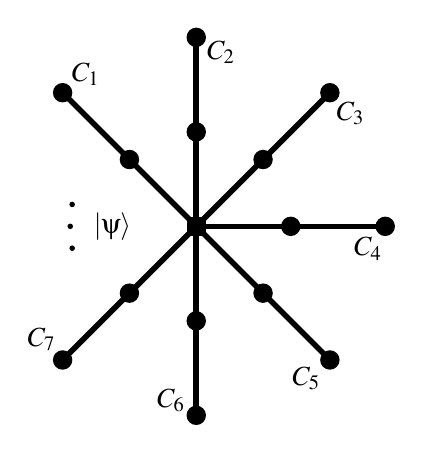
\begin{tikzpicture}  [scale=0.8]
\tikzstyle{every path}=[line width=1pt]
\tikzstyle{every node}=[draw,line width=1pt,inner sep=0]

\tikzstyle{c1}=[rectangle,minimum size=6]

\tikzstyle{d1}=[circle,draw=none,fill,minimum size=2]

\tikzstyle{l7}=[draw=none,circle,minimum size=45]

\draw[black,line width=2pt] (0:0) -- (135:3)
        coordinate[c1,at start] (0)
        coordinate[c1,circle,midway,fill] (1)
        coordinate[c1,circle,at end,fill,label=35:$C_1$] (2);

\draw[black,line width=2pt] (0.center) -- (90:3)
        coordinate[c1,at start] (0)
        coordinate[c1,circle,midway,fill] (3)
        coordinate[c1,circle,at end,fill,label=350:$C_2$] (4);

\draw[black,line width=2pt] (0.center) -- (45:3)
        coordinate[c1,at start] (0)
        coordinate[c1,circle,midway,fill] (5)
        coordinate[c1,circle,at end,fill,label=305:$C_3$] (6);

\draw[black,line width=2pt] (0.center) -- (315:3)
        coordinate[c1,at start] (0)
        coordinate[c1,circle,midway,fill] (9)
        coordinate[c1,circle,at end,fill,label=215:$C_5$] (10);

\draw[black,line width=2pt] (0.center) -- (270:3)
        coordinate[c1,at start] (0)
        coordinate[c1,circle,midway,fill] (11)
        coordinate[c1,circle,at end,fill,label=170:$C_6$] (12);

\draw[black,line width=2pt] (0.center) -- (225:3)
        coordinate[c1,at start] (0)
        coordinate[c1,circle,midway,fill] (13)
        coordinate[c1,circle,at end,fill,label=125:$C_7$] (14);

\draw[black,line width=2pt] (0.center) -- (0:3)
        coordinate[c1,fill,at start] (0)
        coordinate[c1,circle,fill,midway,fill] (7)
        coordinate[c1,circle,,fill,at end,label=260:$C_4$] (8);

\coordinate[l7,label=180:$\vert \psi \rangle$] (0) at (0.center);

\coordinate[d1,black] (.) at (190:2);
\coordinate[d1,black] (.) at (180:2);
\coordinate[d1,black] (.) at (170:2);
\end{tikzpicture}
&
\qquad
\qquad
\qquad
&
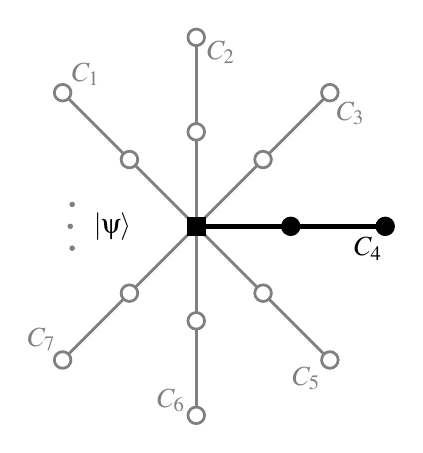
\begin{tikzpicture}  [scale=0.8]
\tikzstyle{every path}=[line width=1pt]
\tikzstyle{every node}=[draw,line width=1pt,inner sep=0]

\tikzstyle{c1}=[rectangle,minimum size=6]

\tikzstyle{d1}=[circle,draw=none,fill,minimum size=2]

\tikzstyle{l7}=[draw=none,circle,minimum size=45]

\draw[gray] (0:0) -- (135:3)
        coordinate[c1,at start] (0)
        coordinate[c1,circle,midway,fill=white] (1)
        coordinate[c1,circle,at end,fill=white,label=35:$C_1$] (2);

\draw[gray] (0.center) -- (90:3)
        coordinate[c1,at start] (0)
        coordinate[c1,circle,midway,fill=white] (3)
        coordinate[c1,circle,at end,fill=white,label=350:$C_2$] (4);

\draw[gray] (0.center) -- (45:3)
        coordinate[c1,at start] (0)
        coordinate[c1,circle,midway,fill=white] (5)
        coordinate[c1,circle,at end,fill=white,label=305:$C_3$] (6);

\draw[gray] (0.center) -- (315:3)
        coordinate[c1,at start] (0)
        coordinate[c1,circle,midway,fill=white] (9)
        coordinate[c1,circle,at end,fill=white,label=215:$C_5$] (10);

\draw[gray] (0.center) -- (270:3)
        coordinate[c1,at start] (0)
        coordinate[c1,circle,midway,fill=white] (11)
        coordinate[c1,circle,at end,fill=white,label=170:$C_6$] (12);

\draw[gray] (0.center) -- (225:3)
        coordinate[c1,at start] (0)
        coordinate[c1,circle,midway,fill=white] (13)
        coordinate[c1,circle,at end,fill=white,label=125:$C_7$] (14);

\draw[black,line width=2pt] (0.center) -- (0:3)
        coordinate[c1,fill,at start] (0)
        coordinate[c1,circle,fill,midway] (7)
        coordinate[c1,circle,fill,at end,label=260:$C_4$] (8);

\coordinate[l7,label=180:$\vert \psi \rangle$] (0) at (0.center);

\coordinate[d1,gray] (.) at (190:2);
\coordinate[d1,gray] (.) at (180:2);
\coordinate[d1,gray] (.) at (170:2);
\end{tikzpicture}
\\
(a)&&(b)
\end{tabular}
\end{center}
\caption{(Color online)
Greechie orthogonality diagram of a star-shaped configuration,
representing a common detector observable $\vert \psi  \rangle \langle  \psi \vert$
with an overlaid two-valued assignment reflecting $v(P_\psi ,\cdot )=1$.
(a) all ``branches'' corresponding to contects are assumed to be equally value definite;
(b) it is assumed that, since the system is prepared in, say, context $C_4$, depicted by a block colored in thick filled black,
only this context is value definite;
all the other (continuity of) contexts are   ``phantom contexts'' colored in gray.
}
\label{2013-KstLip-f5}
\end{figure}

One could be inclined to go one step further and conjecture that
{\em there does not exist any value definite observable outside of a single context.}
This context is defined by the preparation of the state: it consists of
the observable corresponding to $\vert \psi \rangle$,
as well as of the two other orthogonal projectors associated with the two idle detectors that
do not click if $D_\psi $ clicks.
The configuration can be represented by the Greechie orthogonality diagram
depicted in Fig.~\ref{2013-KstLip-f5}(b).
This conjecture is strictly metaphysical with respect to quantum mechanics, because  with our assumptions
it seems that one cannot prove the  sole existence of just one, unique context among the
%%%%CC continuity
continuum of context forming
``$\vert \psi \rangle$'s star.''

Let us mention that one of the authors is inclined to believe in such an existence, another one
is inclined to not believe therein, and the third author has no inclination towards either speculation.

\section*{Acknowledgement} This work was supported in part by Marie Curie FP7-PEOPLE-2010-IRSES Grant RANPHYS.
Part of the work was done while Abbott and Calude were visiting the Institute for Theoretical Physics,
Vienna  University of Technology in September 2013. Calude was also supported by a University of Auckland Grant-in-Aid 2013.
Svozil acknowledges Jeffrey Bub, William Demopoulos, and Christopher Fuchs pointing out similarities to Pitowsky's indeterminacy principle.
%\bibliographystyle{plain}

\appendix*

\section{Detailed Analysis of $f(p_1)$}
\label{sec:appendix}

The proof of Lemma~\ref{lemma:reduction2} relies critically on the analysis of the function $f(p_1) = \iprod{a}{c}$ for $p_1\in \left(\frac{3}{\sqrt{14}},1\right)$.
Here we give further details of this analysis, which was carried out using Wolfram Mathematica 9.0.1.0.

Specifically, we have
$$f(p_1)=\iprod{a}{c}=x_3p_1 + \frac{y_3}{k}(x_2-p_1p_3)- \frac{q_1 z_3}{k q_2}(y_2z_1+y_1z_2),$$
where the constants are defined in terms of $p_1$ as follows:
$$
\alpha_1=\frac{\arccos\sqrt{\frac{2}{3}}}{\arccos\frac{1}{\sqrt{2}}}\raisebox{0.5ex}{,}\phantom{xxx}
\alpha_2=\frac{\arccos\frac{2}{\sqrt{5}}}{\arccos\sqrt{\frac{2}{3}}}\raisebox{0.5ex}{,}\phantom{xxx}
\alpha_3=\frac{\arccos\sqrt{\frac{2}{3}}}{\arccos\sqrt{\frac{2}{5}}}\raisebox{0.5ex}{,}	$$
$$\theta_{a,b}=\arccos p_1,\phantom{xxx}
\theta_{a,v_1}=\alpha_1 \theta_{a,b},\phantom{xxx}
\theta_{a,v_2}=\alpha_2 \theta_{a,v_1},$$
$$q_1=\sqrt{1-p_1^2},\phantom{xxx}
x_1=\cos\theta_{a,v_1},\phantom{xxx}
y_1=\frac{p_1(1-x_1^2)}{q_1 x_1},\phantom{xxx}
z_1=\sqrt{1-x_1^2-y_1^2},$$
$$q_2=\sqrt{1-x_1^2},\phantom{xxx}
x_2=\cos\theta_{a,v_2},\phantom{xxx}
y2=\frac{x_1(1-x_2^2)}{q_2x_2},\phantom{xxx}
z_2=\sqrt{1-x_2^2-y_2^2},$$
$$p_3=p_1 x_2+q_1\frac{y_1y_2-z_1z_2}{q_2},\phantom{xxx}
\theta_{b,v_2}=\arccos p_3,\phantom{xxx}
\theta_{b,c}=\alpha_3\theta_{b,v_2},$$$$
q_3=\sqrt{1-p_3^2},\phantom{xxx}
x_3=\cos\theta_{b,c},\phantom{xxx}
y_3=p_3\frac{(1-x_3^2)}{q_3 x_3},\phantom{xxx}
z_3=\sqrt{1-x_3^2-y_3^2},$$
$$k=\sqrt{\left(\frac{q_1}{q_2}(y_2z_1+y_1z_2)\right)^2+\left(\frac{-p_1}{q_2}(y_2z_1+y_1z_2)\right)^2+\left(\frac{p_1}{q_2}(y_1y_2-z_1z_2)-q_1 x_2\right)^2}.$$

Explicitly writing $f(p_1)$ by completing the substitutions would take several pages, but using Mathematica, we find that the Taylor series expansion around $p_1=1$ is
%\begin{align}
%	f(p_1)=& 1+\frac{(p_1-1)}{\pi^2\acos^2\sqrt{\frac{2}{5}}}\left(\pi^2\left(\acos^2\sqrt{\frac{2}{5}}+\acosh^2\sqrt{\frac{2}{3}} \right)\right.\\
%	&\left. 8\acos\frac{2}{\sqrt{5}}\left(  \right) \right)
%\end{align}
\begin{align*}
	f(p_1)=&
		1+\frac{(p_1-1)}{\pi ^2 \arccos^2\sqrt{\frac{2}{5}}}
	   \left(\pi ^2 \left(\arccos^2\sqrt{\frac{2}{5}}+
	   \arcosh^2\sqrt{\frac{2}{3}}\right)\right.\\
	   &+\left. 8
	   \arccos\frac{2}{\sqrt{5}} \left(
	   \arccos\frac{2}{\sqrt{5}} \left(2
	   \arccos^2\sqrt{\frac{2}{3}}\right.\right.\right.\\
	   &+\left.\left.\left.\sqrt{\left(\pi ^2+16
	   \arcosh^2\sqrt{\frac{2}{3}}\right) \left(
	   \arccos^2\sqrt{\frac{2}{5}}+
	   \arcosh^2\sqrt{\frac{2}{3}}\right)}\right)+4
	   \arccos\sqrt{\frac{2}{3}}\right.\right.\\
	   &\times\left.\left. \sqrt{\left(
	   \arccos^2\sqrt{\frac{2}{5}}+
	   \arcosh^2\sqrt{\frac{2}{3}}\right) \left(
	   \arccos^2\sqrt{\frac{2}{3}}+
	   \arcosh^2\frac{2}{\sqrt{5}}\right)}\right)\right)\\
	   &+\mathcal{O}((p_1-1)^2),
\end{align*}
which numerically simplifies to
$$f(p_1)=1-1.2658(1-p_1)+\mathcal{O}((p_1-1)^2).$$

We calculate $\frac{df}{dp_1}$ from the full expression using Mathematica, but do not give here the resulting function as it is longer yet than the expression for $f(p_1)$.


%merlin.mbs apsrev4-1.bst 2010-07-25 4.21a (PWD, AO, DPC) hacked
%Control: key (0)
%Control: author (0) dotless jnrlst
%Control: editor formatted (1) identically to author
%Control: production of article title (0) allowed
%Control: page (1) range
%Control: year (0) verbatim
%Control: production of eprint (0) enabled
\begin{thebibliography}{9}%
\makeatletter
\providecommand \@ifxundefined [1]{%
 \@ifx{#1\undefined}
}%
\providecommand \@ifnum [1]{%
 \ifnum #1\expandafter \@firstoftwo
 \else \expandafter \@secondoftwo
 \fi
}%
\providecommand \@ifx [1]{%
 \ifx #1\expandafter \@firstoftwo
 \else \expandafter \@secondoftwo
 \fi
}%
\providecommand \natexlab [1]{#1}%
\providecommand \enquote  [1]{``#1''}%
\providecommand \bibnamefont  [1]{#1}%
\providecommand \bibfnamefont [1]{#1}%
\providecommand \citenamefont [1]{#1}%
\providecommand \href@noop [0]{\@secondoftwo}%
\providecommand \href [0]{\begingroup \@sanitize@url \@href}%
\providecommand \@href[1]{\@@startlink{#1}\@@href}%
\providecommand \@@href[1]{\endgroup#1\@@endlink}%
\providecommand \@sanitize@url [0]{\catcode `\\12\catcode `\$12\catcode
  `\&12\catcode `\#12\catcode `\^12\catcode `\_12\catcode `\%12\relax}%
\providecommand \@@startlink[1]{}%
\providecommand \@@endlink[0]{}%
\providecommand \url  [0]{\begingroup\@sanitize@url \@url }%
\providecommand \@url [1]{\endgroup\@href {#1}{\urlprefix }}%
\providecommand \urlprefix  [0]{URL }%
\providecommand \Eprint [0]{\href }%
\providecommand \doibase [0]{http://dx.doi.org/}%
\providecommand \selectlanguage [0]{\@gobble}%
\providecommand \bibinfo  [0]{\@secondoftwo}%
\providecommand \bibfield  [0]{\@secondoftwo}%
\providecommand \translation [1]{[#1]}%
\providecommand \BibitemOpen [0]{}%
\providecommand \bibitemStop [0]{}%
\providecommand \bibitemNoStop [0]{.\EOS\space}%
\providecommand \EOS [0]{\spacefactor3000\relax}%
\providecommand \BibitemShut  [1]{\csname bibitem#1\endcsname}%
\let\auto@bib@innerbib\@empty
%</preamble>
\bibitem [{\citenamefont {Specker}(1960)}]{specker-60}%
  \BibitemOpen
  \bibfield  {author} {\bibinfo {author} {\bibfnamefont {Ernst}\ \bibnamefont
  {Specker}},\ }\bibfield  {title} {\enquote {\bibinfo {title} {{D}ie {L}ogik
  nicht gleichzeitig entscheidbarer {A}ussagen},}\ }\href {\doibase
  10.1111/j.1746-8361.1960.tb00422.x} {\bibfield  {journal} {\bibinfo
  {journal} {Dialectica}\ }\textbf {\bibinfo {volume} {14}},\ \bibinfo {pages}
  {239--246} (\bibinfo {year} {1960})},\ \Eprint
  {http://arxiv.org/abs/http://arxiv.org/abs/1103.4537}
  {http://arxiv.org/abs/1103.4537} \BibitemShut {NoStop}%
\bibitem [{\citenamefont {Kochen}\ and\ \citenamefont
  {Specker}(1967)}]{kochen1}%
  \BibitemOpen
  \bibfield  {author} {\bibinfo {author} {\bibfnamefont {Simon}\ \bibnamefont
  {Kochen}}\ and\ \bibinfo {author} {\bibfnamefont {Ernst~P.}\ \bibnamefont
  {Specker}},\ }\bibfield  {title} {\enquote {\bibinfo {title} {The problem of
  hidden variables in quantum mechanics},}\ }\href {\doibase
  10.1512/iumj.1968.17.17004} {\bibfield  {journal} {\bibinfo  {journal}
  {Journal of Mathematics and Mechanics (now Indiana University Mathematics
  Journal)}\ }\textbf {\bibinfo {volume} {17}},\ \bibinfo {pages} {59--87}
  (\bibinfo {year} {1967})}\BibitemShut {NoStop}%
\bibitem [{\citenamefont {Abbott}\ \emph {et~al.}(2012)\citenamefont {Abbott},
  \citenamefont {Calude}, \citenamefont {Conder},\ and\ \citenamefont
  {Svozil}}]{2012-incomput-proofsCJ}%
  \BibitemOpen
  \bibfield  {author} {\bibinfo {author} {\bibfnamefont {Alastair~A.}\
  \bibnamefont {Abbott}}, \bibinfo {author} {\bibfnamefont {Cristian~S.}\
  \bibnamefont {Calude}}, \bibinfo {author} {\bibfnamefont {Jonathan}\
  \bibnamefont {Conder}}, \ and\ \bibinfo {author} {\bibfnamefont {Karl}\
  \bibnamefont {Svozil}},\ }\bibfield  {title} {\enquote {\bibinfo {title}
  {Strong {K}ochen-{S}pecker theorem and incomputability of quantum
  randomness},}\ }\href {\doibase 10.1103/PhysRevA.86.062109} {\bibfield
  {journal} {\bibinfo  {journal} {Physical Review A}\ }\textbf {\bibinfo
  {volume} {86}},\ \bibinfo {pages} {062109} (\bibinfo {year} {2012})},\
  \Eprint {http://arxiv.org/abs/arXiv:1207.2029} {arXiv:1207.2029} \BibitemShut
  {NoStop}%
\bibitem [{\citenamefont {Pitowsky}(1998)}]{pitowsky:218}%
  \BibitemOpen
  \bibfield  {author} {\bibinfo {author} {\bibfnamefont {Itamar}\ \bibnamefont
  {Pitowsky}},\ }\bibfield  {title} {\enquote {\bibinfo {title} {Infinite and
  finite {G}leason's theorems and the logic of indeterminacy},}\ }\href
  {\doibase 10.1063/1.532334} {\bibfield  {journal} {\bibinfo  {journal}
  {Journal of Mathematical Physics}\ }\textbf {\bibinfo {volume} {39}},\
  \bibinfo {pages} {218--228} (\bibinfo {year} {1998})}\BibitemShut {NoStop}%
\bibitem [{\citenamefont {Hrushovski}\ and\ \citenamefont
  {Pitowsky}(2004)}]{hru-pit-2003}%
  \BibitemOpen
  \bibfield  {author} {\bibinfo {author} {\bibfnamefont {Ehud}\ \bibnamefont
  {Hrushovski}}\ and\ \bibinfo {author} {\bibfnamefont {Itamar}\ \bibnamefont
  {Pitowsky}},\ }\bibfield  {title} {\enquote {\bibinfo {title}
  {Generalizations of {K}ochen and {S}pecker's theorem and the effectiveness of
  {G}leason's theorem},}\ }\href {\doibase 10.1016/j.shpsb.2003.10.002}
  {\bibfield  {journal} {\bibinfo  {journal} {Studies in History and Philosophy
  of Science Part B: Studies in History and Philosophy of Modern Physics}\
  }\textbf {\bibinfo {volume} {35}},\ \bibinfo {pages} {177­194} (\bibinfo
  {year} {2004})},\ \Eprint {http://arxiv.org/abs/quant-ph/0307139}
  {quant-ph/0307139} \BibitemShut {NoStop}%
\bibitem [{\citenamefont {{von Neumann}}(1955)}]{v-neumann-55}%
  \BibitemOpen
  \bibfield  {author} {\bibinfo {author} {\bibfnamefont {John}\ \bibnamefont
  {{von Neumann}}},\ }\href@noop {} {\emph {\bibinfo {title} {Mathematical
  Foundations of Quantum Mechanics}}}\ (\bibinfo  {publisher} {Princeton
  University Press},\ \bibinfo {address} {Princeton, NJ},\ \bibinfo {year}
  {1955})\BibitemShut {NoStop}%
\bibitem [{\citenamefont {Birkhoff}\ and\ \citenamefont {{von
  Neumann}}(1936)}]{birkhoff-36}%
  \BibitemOpen
  \bibfield  {author} {\bibinfo {author} {\bibfnamefont {Garrett}\ \bibnamefont
  {Birkhoff}}\ and\ \bibinfo {author} {\bibfnamefont {John}\ \bibnamefont {{von
  Neumann}}},\ }\bibfield  {title} {\enquote {\bibinfo {title} {The logic of
  quantum mechanics},}\ }\href {\doibase 10.2307/1968621} {\bibfield  {journal}
  {\bibinfo  {journal} {Annals of Mathematics}\ }\textbf {\bibinfo {volume}
  {37}},\ \bibinfo {pages} {823--843} (\bibinfo {year} {1936})}\BibitemShut
  {NoStop}%
\bibitem [{\citenamefont {Kochen}\ and\ \citenamefont
  {Specker}(1965{\natexlab{a}})}]{kochen2}%
  \BibitemOpen
  \bibfield  {author} {\bibinfo {author} {\bibfnamefont {Simon}\ \bibnamefont
  {Kochen}}\ and\ \bibinfo {author} {\bibfnamefont {Ernst~P.}\ \bibnamefont
  {Specker}},\ }\bibfield  {title} {\enquote {\bibinfo {title} {Logical
  structures arising in quantum theory},}\ }in\ \href@noop {} {\emph {\bibinfo
  {booktitle} {Symposium on the Theory of Models, Proceedings of the 1963
  International Symposium at Berkeley}}}\ (\bibinfo  {publisher} {North
  Holland},\ \bibinfo {address} {Amsterdam},\ \bibinfo {year} {1965})\ pp.\
  \bibinfo {pages} {177--189}\BibitemShut {NoStop}%
\bibitem [{\citenamefont {Kochen}\ and\ \citenamefont
  {Specker}(1965{\natexlab{b}})}]{kochen3}%
  \BibitemOpen
  \bibfield  {author} {\bibinfo {author} {\bibfnamefont {Simon}\ \bibnamefont
  {Kochen}}\ and\ \bibinfo {author} {\bibfnamefont {Ernst~P.}\ \bibnamefont
  {Specker}},\ }\bibfield  {title} {\enquote {\bibinfo {title} {The calculus of
  partial propositional functions},}\ }in\ \href@noop {} {\emph {\bibinfo
  {booktitle} {Proceedings of the 1964 International Congress for Logic,
  Methodology and Philosophy of Science, Jerusalem}}}\ (\bibinfo  {publisher}
  {North Holland},\ \bibinfo {address} {Amsterdam},\ \bibinfo {year} {1965})\
  pp.\ \bibinfo {pages} {45--57}\BibitemShut {NoStop}%
\end{thebibliography}%

%\bibliography{svozil.bib}
\end{document}
